This chapter gives a brief overview of what messaging is and how it can be used for system integration purposes. It introduces various messaging patterns which will be used by the technological integration of chapter 4 and 5.
The content of this chapter is based on the book \textit{Enterprise Integration Patterns} by \textcite{EIP}.

\section{Messaging}

Messaging is an asynchronous system-to-system communication, delivering packages of data called messages trough channels. Messages can contain any structured data like strings, arrays or objects. It is up to the sender and receiver to determine and understand its content.

Channels can be seen as a collection or array of messages, accessible to interested systems. Channels have a direction in a sense, that no system simultaneously writes to and reads from a channel. Therefore, by one system writing messages to a channel and another system reading them, a message and data flow can be established.

Depending on the use case, the flow and destination of messages might have to be determined during operation. Therefore, various message routing components exist. Their purpose is to transfer messages from an inbound channel to one or more outbound channels, depending on predefined or dynamic rules.

During the routing of messages between systems, the content of messages might have to be modified. Therefore various message transformation components exist. Their purpose is to consume messages from an inbound channel, modify their content based on predefined or dynamic rules and publish the modified message on a outbound channel.

"\textit{A messaging system manages messaging the way a database system manages data persistence}" \cite[p. 31]{EIP}. Configuring a messaging system involves definition of available channels, the type of messages they exchange, their connection between systems, the message flow and where necessary the insertion of routing and transformation components.

Depending on the messaging system solution, additional features can be configured to increase performance, stability, failure safety and more. If properly configured, the messaging system operates reliably, handles unreliable network connections and persistently store messages in case of a system crash.

\section{Messaging Integration}

One use case for a messaging system is integration.

The main benefit of messaging for integration is, that it enables systems to share services and data in a decoupled way. Neither system, whether sending or receiving messages, needs to be aware of each other. 

During configuration of the messaging system, datatype channels can be defined. On these channels, only messages with the same content are exchanged. Using message transformation components, messages placed on a datatype channel can be translated to follow a canonical data model.

Systems consuming messages from datatype channels can individually assign a purpose to channels independent from the sending system. As a result of the canonical data model, receiving systems can also choose a data structure independent from the sending system.

As channels are able to function as a message buffer, sender and receiver of messages do not even have to be running at the same time.

\section{Messaging Patterns}

In the book "\textit{Enterprise Integration Patterns}" by \cite{EIP} multiple patterns for designing messaging systems are presented. This section gives a brief overview of patterns relevant for the thesis.

\paragraph{Message}

\begin{center}
    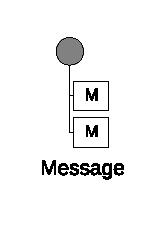
\includegraphics[scale=0.6]{Diagrams/Messaging/1. Message.pdf}
\end{center}

\paragraph{Channel}

\begin{center}
    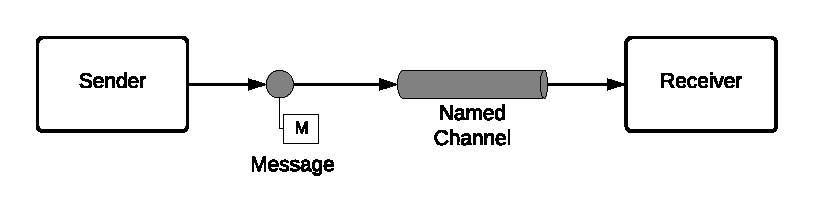
\includegraphics[scale=0.6]{Diagrams/Messaging/2. Channel.pdf}
\end{center}

\begin{center}
    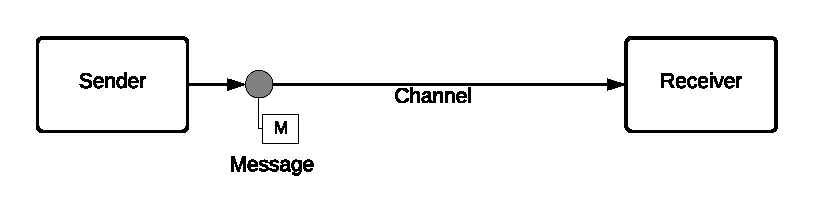
\includegraphics[scale=0.6]{Diagrams/Messaging/3. Channel.pdf}
\end{center}

\paragraph{Messaging Adapter}

\begin{center}
    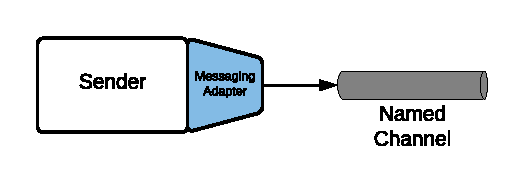
\includegraphics[scale=0.6]{Diagrams/Messaging/4. Messaging Adapter.pdf}
\end{center}

\paragraph{Message Router}

\begin{center}
    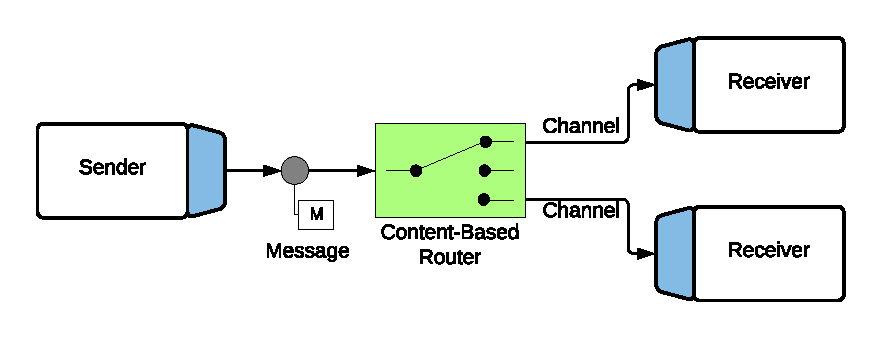
\includegraphics[scale=0.6]{Diagrams/Messaging/5. Message Router.pdf}
\end{center}

\paragraph{Message Translator}

\begin{center}
    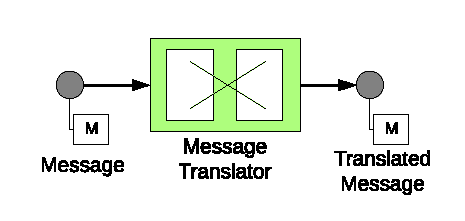
\includegraphics[scale=0.6]{Diagrams/Messaging/6. Message Translator.pdf}
\end{center}

\begin{center}
    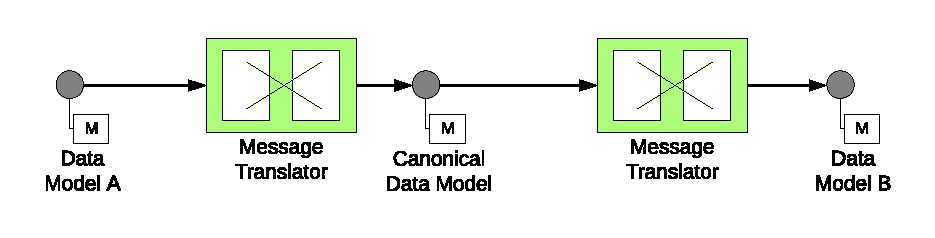
\includegraphics[scale=0.6]{Diagrams/Messaging/7. Message Translator.pdf}
\end{center}

\paragraph{Message Filter}

\begin{center}
    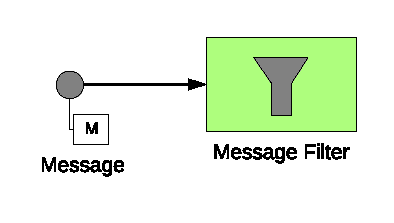
\includegraphics[scale=0.6]{Diagrams/Messaging/8. Message Filter.pdf}
\end{center}

\paragraph{Content Enricher}

\begin{center}
    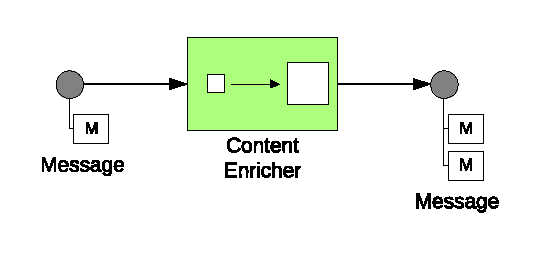
\includegraphics[scale=0.6]{Diagrams/Messaging/9. Content Enricher.pdf}
\end{center}

\paragraph{Content Filter}

\begin{center}
    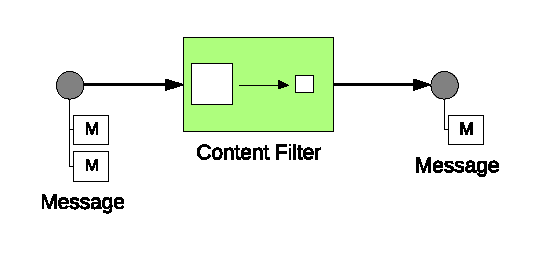
\includegraphics[scale=0.6]{Diagrams/Messaging/10. Content Filter.pdf}
\end{center}

\paragraph{Message Store}

\begin{center}
    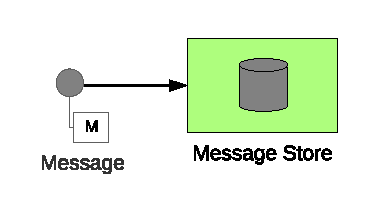
\includegraphics[scale=0.6]{Diagrams/Messaging/11. Message Store.pdf}
\end{center}

